\documentclass{article}
\usepackage[T2A]{fontenc}
\usepackage[utf8]{inputenc}
\usepackage[russian]{babel}
\usepackage{graphicx}
\usepackage{graphicx}
\DeclareGraphicsExtensions{.pdf,.png,.jpg}

\newcommand{\university}{Национальный исследовательский Университет ИТМО}
\newcommand{\mfaculty}{Мегафакультет информационных и трансляционных технологий}
\newcommand{\faculty}{Факультет инфокоммуникационных технологий}
\newcommand{\city}{Санкт-Петербург}
\newcommand{\docname}{Курсовая работа}
\newcommand{\subject}{Инфокоммуникационные технологии}
\newcommand{\tutorname}{Н.Н. Горлушкина}
\newcommand{\studentname}{А.А. Зубенко}
\newcommand{\group}{K3141}

\begin{document}
\begin{titlepage}	% начало титульной страницы

	\begin{center}		% выравнивание по центру

		\large \university \\ 
		\large \mfaculty \\
		\large \faculty \\[5cm]
		% название института, затем отступ 6см

		\huge \subject \\[0.5cm] % название работы, затем отступ 0,5см
		\large \docname \num \\[4.1cm]
		 %\large Разработка методов обучения с подкреплением\\[5cm]

	\end{center}


	\begin{flushright} % выравнивание по правому краю
		\begin{minipage}{0.25\textwidth} % врезка в половину ширины текста
			\begin{flushleft} % выровнять её содержимое по левому краю

				\large\textbf{Работу выполнил:}\\
				\large \studentname \\
				\large {Группа:} \group \\

				\large \textbf{Преподаватель: }\\
				\large \tutorname

			\end{flushleft}
		\end{minipage}
	\end{flushright}

	\vfill % заполнить всё доступное ниже пространство

	\begin{center}
		\large \city \\
		\large \the\year % вывести дату
	\end{center} % закончить выравнивание по центру

\end{titlepage} % конец титульной страницы

\vfill % заполнить всё доступное ниже пространство

\tableofcontents

\newpage
\begin{center}
	\textbf{ИТОГИ КУРСОВОГО ПРОЕКТА}
\end{center} % закончить выравнивание по центру

\section{Задача 1.Изучить ресурсы, предоставляющие информацию о вакансиях.}

Первое, сделанное нашей командой - подбор ресурсов, которые будут использоваться в дальнейшем. Для изучения мы выбрали следующие источники:
\begin{itemize}
  \item https://russia.trud.com/salary/692.html - сервис, содержащий информацию по основным направлениям разработки ПО, статистику по уровню заработной платы и диаграммы распределения вакансий по регионам;
  \item https://www.kv.by/post/1059800-rynok-truda-v-it-realii-po-itogam-i-kvartala-2020-goda - наглядные мировые тенденции в IT. Предоставлена информация о наиболее перспективных и высокооплачиваемых направлениях в области разработки;
  \item https://career.habr.com/ - сервис для поиска работы с возможностью ранжирования по популярности вакансий, наличие актуальной информации о заработной плате;
\end{itemize}

Данные сервисы содержат статистику по мировым и Российским тенденциям в IT-сфере, диаграммы распределения вакансий по регионам, а также уровень заработной платы в различных областях разработки. 

\newpage
\section{Задача 2.Выявить, какие специалисты востребованы на рынке труда IT и какие стеки технологий требуются в данных вакансиях, популярность языков программирования.}

Для понимания, в каких специализациях стоит развиваться молодым специалистам, мы провели анализ сервисов по поиску работы и изучили статистику. По полученным данным к 1 кварталу текущего года самыми востребованными вакансиями являются QA Engineer, Java и PHP разработчик, а также Frontend разработчик. 

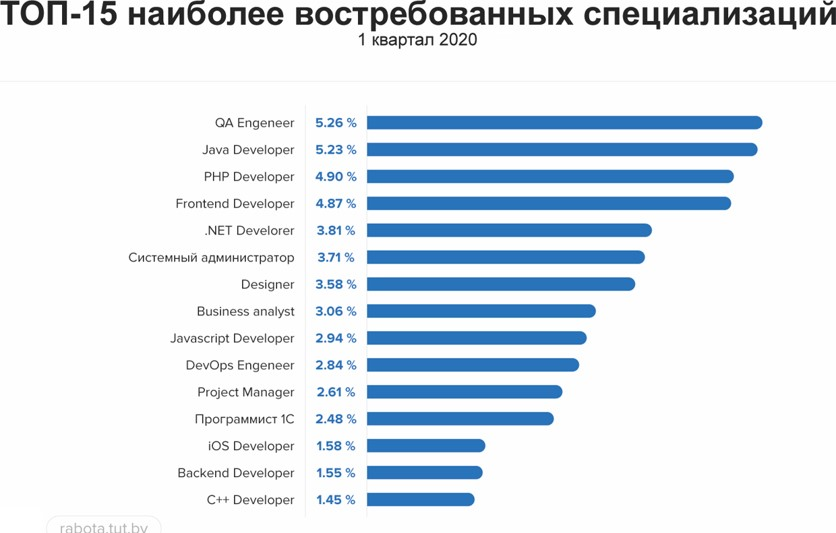
\includegraphics[width=\textwidth]{Images/1.jpg}

Наиболее популярными стеками являются Java, sql, javascript, в то время как kafka и elasticsearch далеко не так популярны.

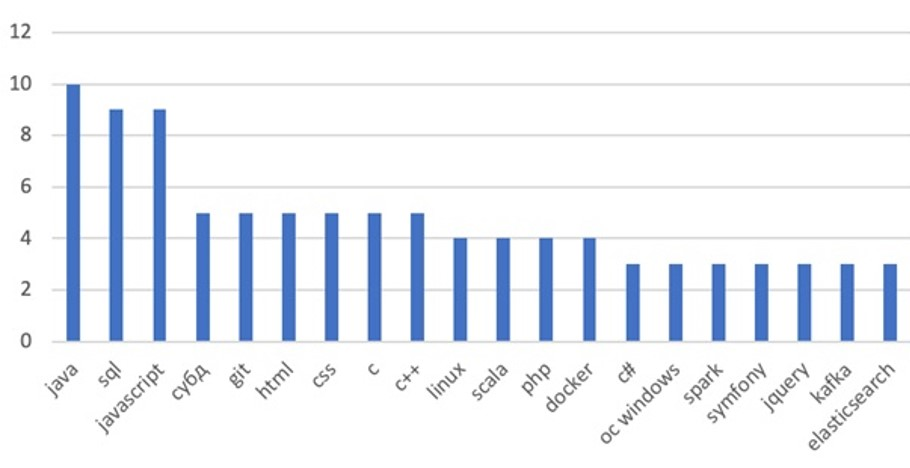
\includegraphics[width=\textwidth]{Images/2.jpg}

Но для успешного поиска работы необходимо знать не только востребованные на рынке труда специализации, а также уровень заработных плат в стране и близлежащих странах. Как можно заметить, в большей части регионов средняя заработная плата составляет 100 000 рублей.

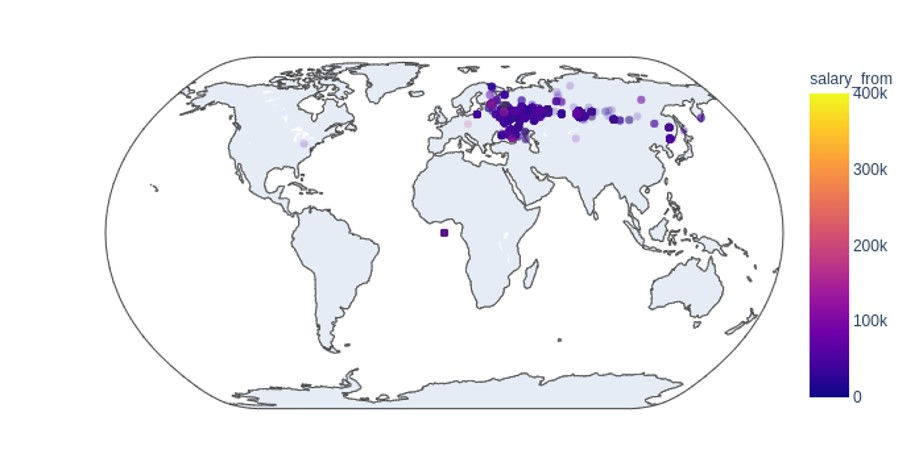
\includegraphics[width=\textwidth]{Images/3.jpg}

Уровень заработной платы в различных регионах страны не менее важен. Так, например, в Москве средний уровень зарплаты в сфере IT составляет 150 000 рублей, в Санкт-Петербурге 120 000 рублей, а в Челябинске 60 000 рублей.

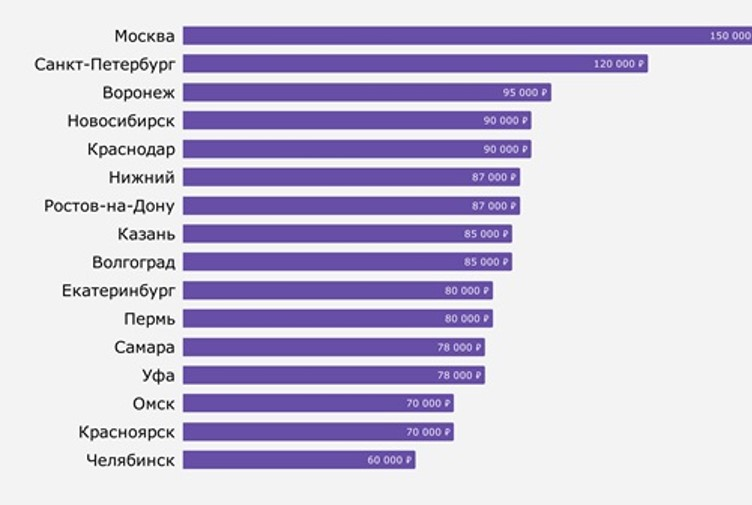
\includegraphics[width=\textwidth]{Images/4.jpg}

Когда молодой специалист определился со своей будущей профессией, ему полезно узнать средний уровень заработной платы в его специальности, а также ее изменения в течении года, чтобы понимать примерный уровень своего будущего заработка. 
Например, уровень средней заработной платы Java-разработчика за последний год варьировался от 100 до 130 тысяч рублей. К данному моменту уровень оплаты вырос, следовательно, необходимость в специалистах возросла.

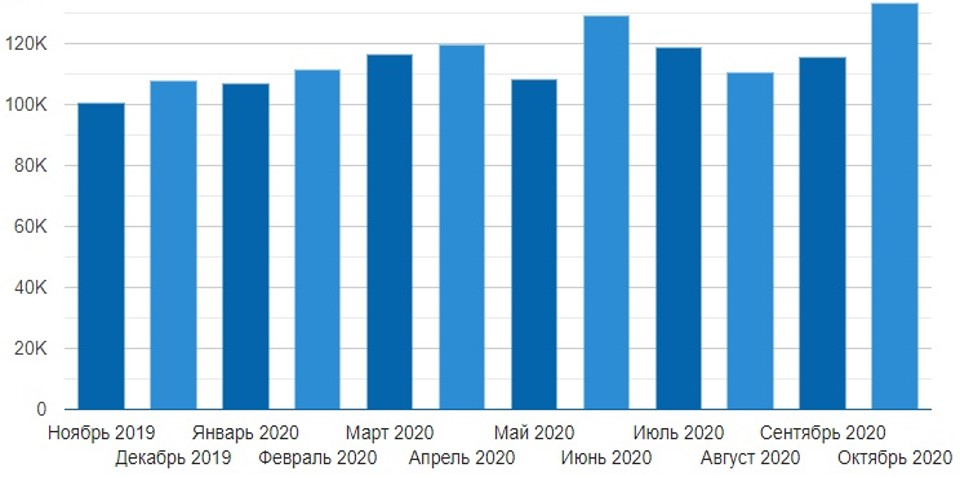
\includegraphics[width=\textwidth]{Images/5.jpg}

При поиске работы также важно знать необходимый стаж работы, который компании требуют от специалистов. Используя сайт headhunter.ru, команда собрала данные по 38 000 вакансий, а позже выбрала оттуда вакансии, связанные с IT. По полученным данным, от IT-специалистов в большинстве случаев требуется опыт работы от 1 года, а 13 процентов работодателей не требуют опыта вовсе.

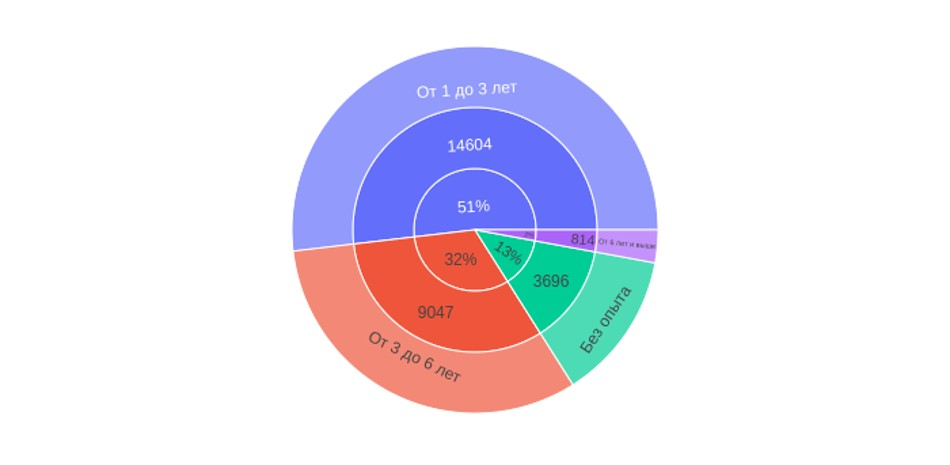
\includegraphics[width=\textwidth]{Images/6.1.jpg}

В сфере разработки же без опыта работы возьмут лишь на 5 процентов из всех предложенных вакансий, со стажем от 1 до 3 лет есть почти 6000 вариантов работы, а меньше всего, как и в случае с IT-сферой в целом, требуется специалистов, проработавших 6 и более лет.   

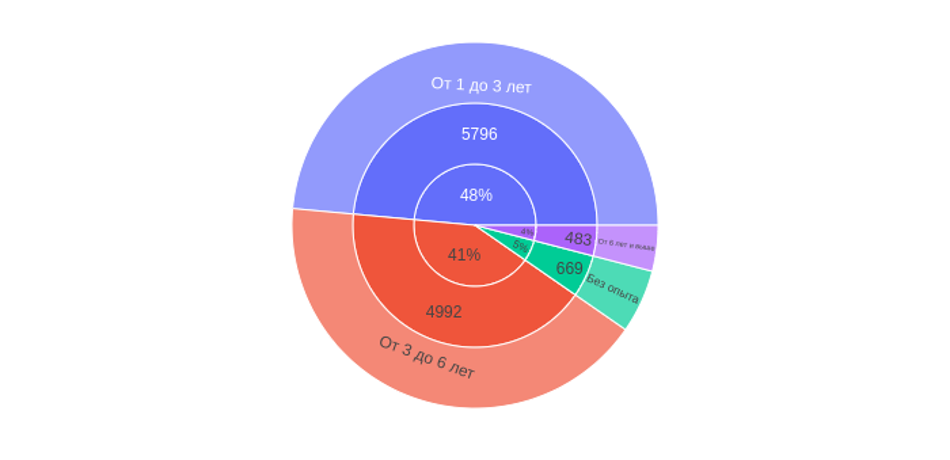
\includegraphics[width=\textwidth]{Images/6.2.png}

Как можно заметить, самая большая необходимость в senior-разработчиках, то есть в людях, которые стали уже действительно хорошими разработчиками и знают свое дело. Middle-разработчиков тоже требуется немало, ведь они уже обладают необходимыми знаниями для участий в проктах. А вот Junior’ов требуется намного меньше.

\newpage
\section{Заключение}

Изучив ресурсы по поиску работы, сайты со статистикой по уровню заработных плат и востребованность специалистов в последнее время, мы пришли к следующим выводам:
\begin{itemize}
  \item Востребованы Java, JavaScript и SQL разработчики, а также QA Engineering;
  \item Самыми высокооплачиваемыми должностями в России являются iOS разработчик, Java разработчик и ведущий специалист;
  \item Больше всего вакансий молодым специалистам доступно в Московской и Ленинградской области, республике Крым.
\end{itemize}
\end{document}
